\documentclass[conference]{IEEEtran}
\usepackage{fancyhdr}
\usepackage{multirow}
\usepackage{amsmath}
\usepackage{graphicx}
\usepackage{cite}
\usepackage{amsfonts}
\usepackage{listings}
\usepackage[colorlinks=true,
            urlcolor  = blue,
            citecolor = red]{hyperref}

\lstset{language=Python}
\setlength{\headheight}{15.2pt}
\pagestyle{fancy}
\renewcommand{\headrulewidth}{0pt} % no line in header area
\fancyhead{}
\lhead{Mini-Project \#3}
\chead{Modified Handwritten Digits Classification}
\rhead{COMP 598}
\fancyfoot{}


\author{David Rapoport, Zafarali Ahmed, Pascale Gourdeau\\Team Name: KernelTrix}
\title{COMP-598 Mini-Project \#3\\Modified Handwritten Digits Classification}
\date{\today}
\begin{document}
\maketitle

\section{Introduction}

Image classification tasks are numerous, and one of the most common being the handwritten digits classification, which has been used as a benchmark in the past thirty years to compare different methods and models\cite{LeCun90} \cite{MNIST_Original}. 

Such tasks have gained a lot of popularity in the past decade, mainly due to advances in the machine learning community involving algorithms that require little to no feature extraction methods before classification. For example, performance on face recognition tasks reached new heights this year, when Google reveiled its FaceNet system which achieved a 99.63\% accuracy 	on the Labeled Faces in the Wild (LFW) dataset\cite{FaceNet}.


Our work explores the performance of four classifiers, namely Logistic Regression, Support Vector Machines, Feed-Forward Neural Network and Convolution Neural Network, on a modified handwritten digits dataset. A main contribution of our work is a comparison between linear classifiers, whose poor performances are attributed to their model simplicity, and layered convolution networks, which have the ability to capture the task's complexity.



\section{Related Work}

The MNIST database of handwritten digits\cite{MNIST_Original} is often used as a baseline to compare performance of different classifiers. Past work on this dataset \cite{MNIST_Original} \cite{LeCun90} \cite{CNN_committees} presents very low error rates, going as low as 0.27\%. Various classifiers have been used throughout the years, ranging from simple models (1-layer neural networks and $k$-Nearest Neighbours) to very complex ones (committees of convolution neural networks).

Work has also been recently done in \cite{modifiedMNIST} demonstrating high performance on the more challenging task of classifying modified digits, where the images undergo a series of transformations, discussed in details in the following section. The error rate is of 3.19\%, which is remarkable considering how different original and modified images are.

\section{Data}

The dataset was obtained from the \href{https://inclass.kaggle.com/c/modified-digits}{Kaggle Competition Website}. A sampling of some digits can be seen in Fig 1, showcasing the apparent difficulty of the task: distinguishing digits proves to be hard even for the human eye.In particular, we expect the digits $6$ and $9$ to be almost indistinguishable, as the images undergo rotation.

The modification of the MNIST \cite{MNIST_Original} database was made by 
\begin{enumerate}
\item Embossing 
\item A rotation by a random angle sampled in $[0,360)$
\item Rescaling from $28\times28$ to $48\times48$ pixels
\item Random texturing, where the pattern is overlayed on the background
\end{enumerate}

\begin{figure}[h]
		\label{MNISTSample1}
	\centering
	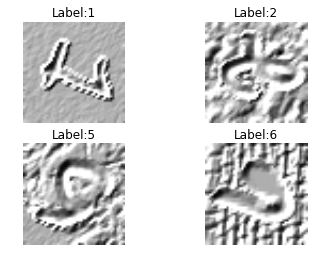
\includegraphics[scale=0.50]{sample_of_images.png}
	\caption{A sampling of the modified MNIST database. It is interesting to notice that the last digit is a 6, even though to the human eye it appears to be a 9.}
\end{figure}

\section{Methodology}

We used the \href{http://www.numpy.org/}{NumPy package} and the \href{http://www.scikit-learn.org/}{scikit-learn library} to perform feature extraction and selection, implement our classifiers, and analyse our results. 

To implement the advanced Convolution Neural Networks we used the \href{http://pythonhosted.org/nolearn/}{nolearn} package that allows easy layering of neural networks found in \href{http://lasagne.readthedocs.org/}{Lasagne}.

\subsection{Dimensionality Reduction}

We explored both Principal Component Analysis (PCA) and scaling the data as methods of dimensionality reduction and feature preprocessing. 

Principal Component analysis is a dimensionality reduction technique which tries to find a pair of linear transformations $f:\mathbb{R}^m\rightarrow\mathbb{R}^p$ and $g:\mathbb{R}^p\rightarrow\mathbb{R}^m$ where $p\leq m$ and for the corresponding matrices $F=G^T$. 
Solving
$$\arg\min_{F,G}\Sigma_{i=0}^N\|x_i-G\times F\times x_i\|^2$$
allows us to recover $F$ and $G$, and thus go from $m$ to $p$ dimensions. 
Scikit-learn's Incremental PCA, which performs PCA in steps, allowed us to avoid a memory blow up. 

We also performed standard scaling so that all features would be distributed according to $\mathcal{N}=\left(\mu=0,\sigma=1\right)$. This also simplified the merging of the modified and orignial digits datasets, as we noticed that the original MNIST dataset took values of 0 and 255 while the modified MNIST dataset took values between 0 and 1.

We performed a GridSearch on different values of p to use as the projected dimensionality of the data after applying PCA, and with and without scaling. The results are in Fig \ref{gridsearchpca} in the Results section.

\subsection{Generating Additional Data}

As per the suggestions of Patrice Simard et al. \cite{Simard} we decided to augment our learners with extra data. The data generated came from two different sources and the effect of the addition of either supplementary dataset is explored later in this paper.

\begin{figure}[h]
	\centering
	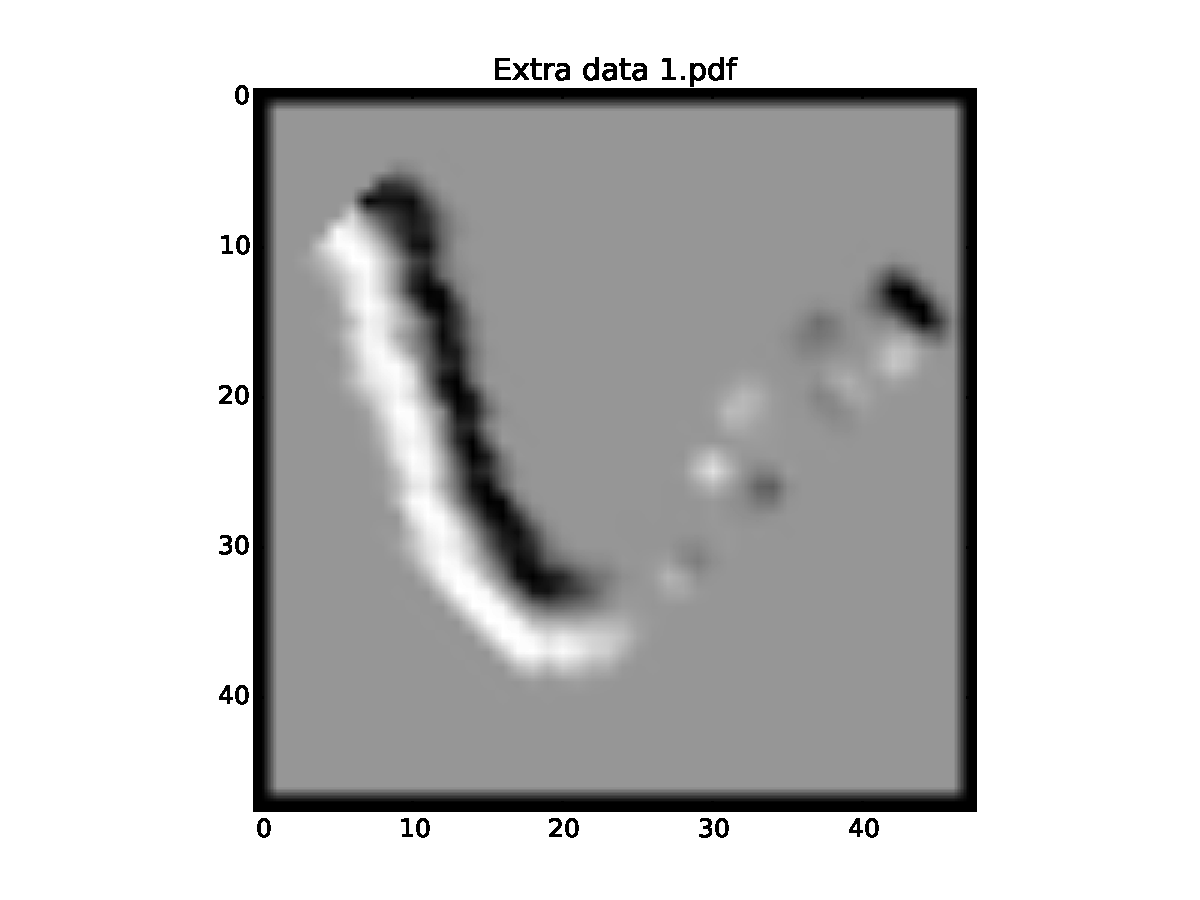
\includegraphics[scale=0.15]{Extradata1.pdf}
	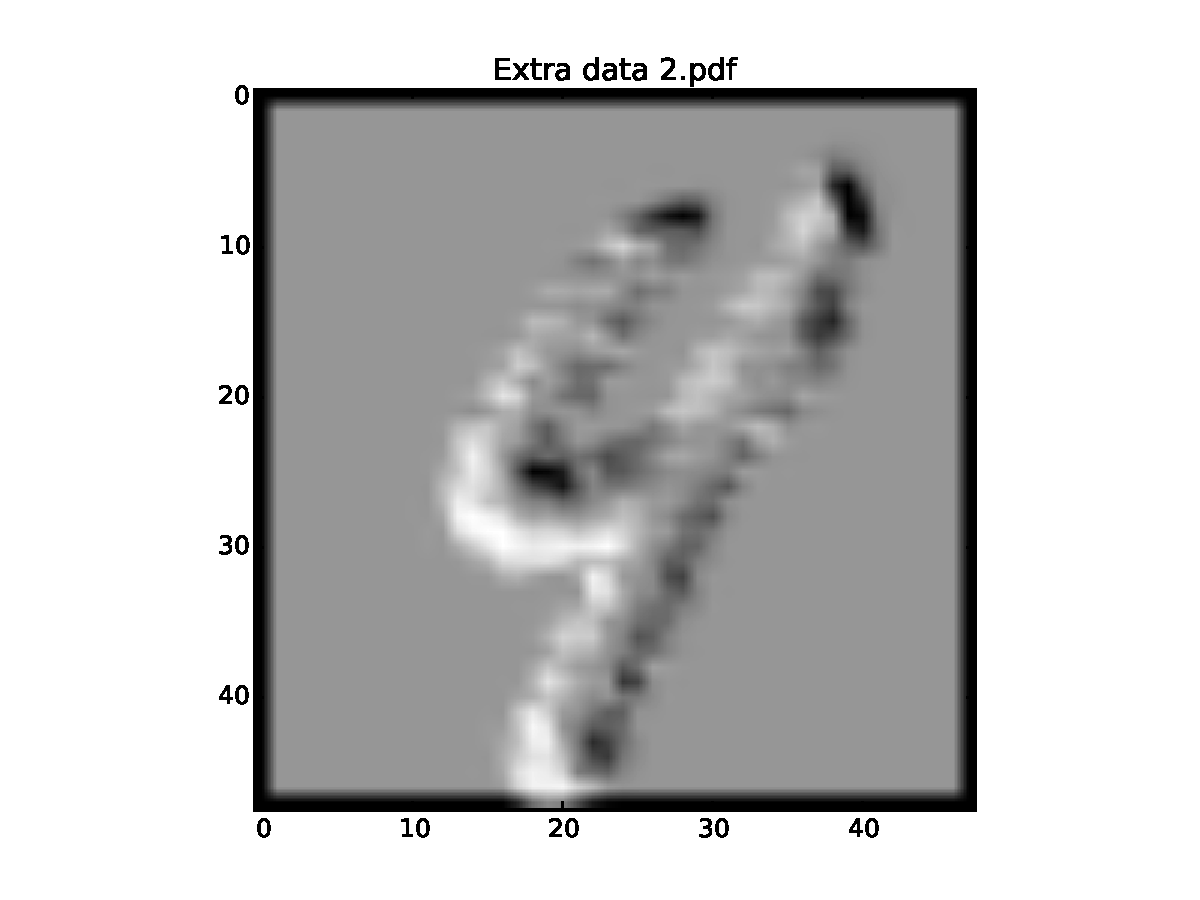
\includegraphics[scale=0.15]{Extradata2.pdf}
	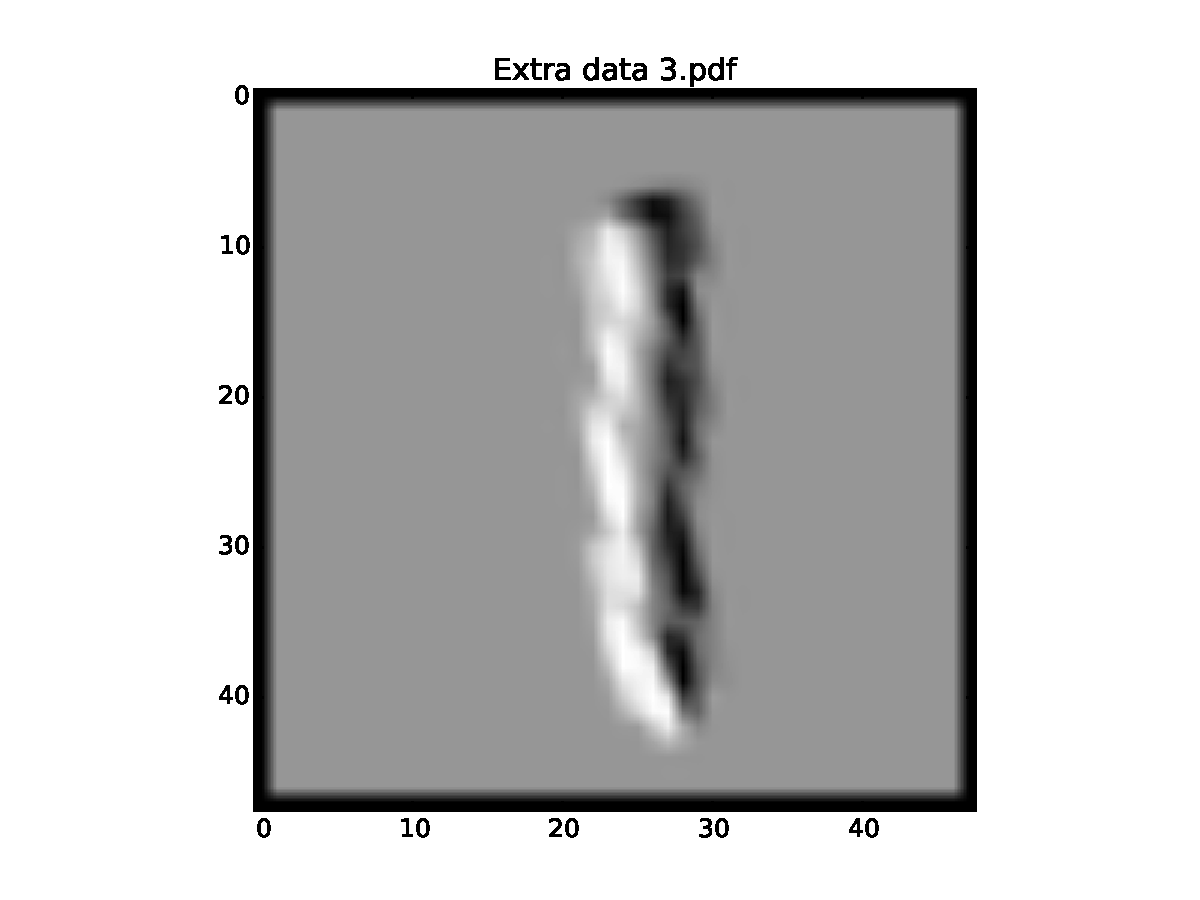
\includegraphics[scale=0.15]{Extradata3.pdf}
	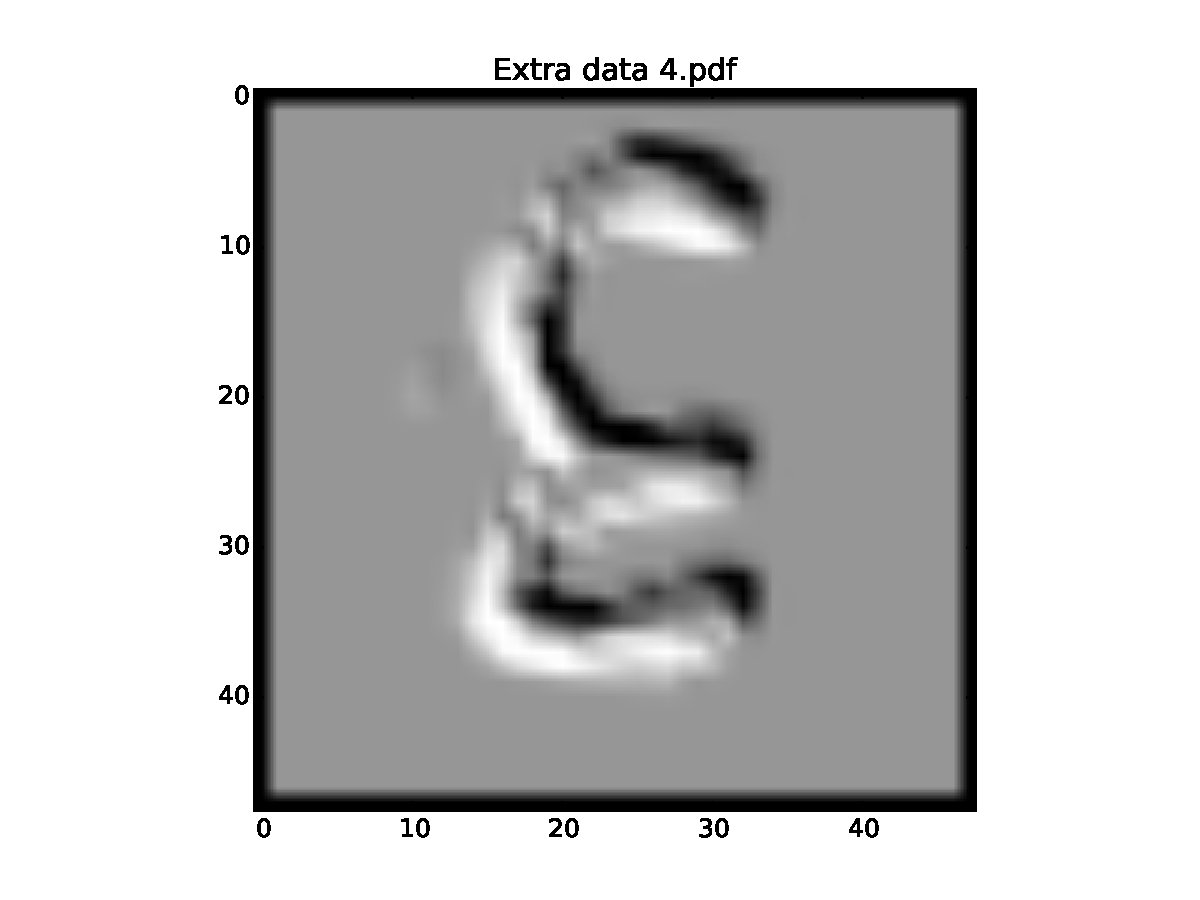
\includegraphics[scale=0.15]{Extradata4.pdf}
	\caption{Four example image from the "Extra Digits" dataset}
	\label{ExtraData}
\end{figure}

The first additional datasource involved transformations of the original MNIST dataset. We will refer to this dataset as "Extra Digits" throughout the rest of the paper. We performed the following transformations as described in the data section: embossing, rescaling and rotating. 
We attempted to add a pattern to the new image as in the modified MNIST dataset, but were unable to find a pattern which we felt maintained the integrity of the image in a way which the patterns used in the modified MNIST dataset did. An example of images from the dataset is shown in Fig \ref{ExtraData}

\begin{figure}[h]
	\centering
	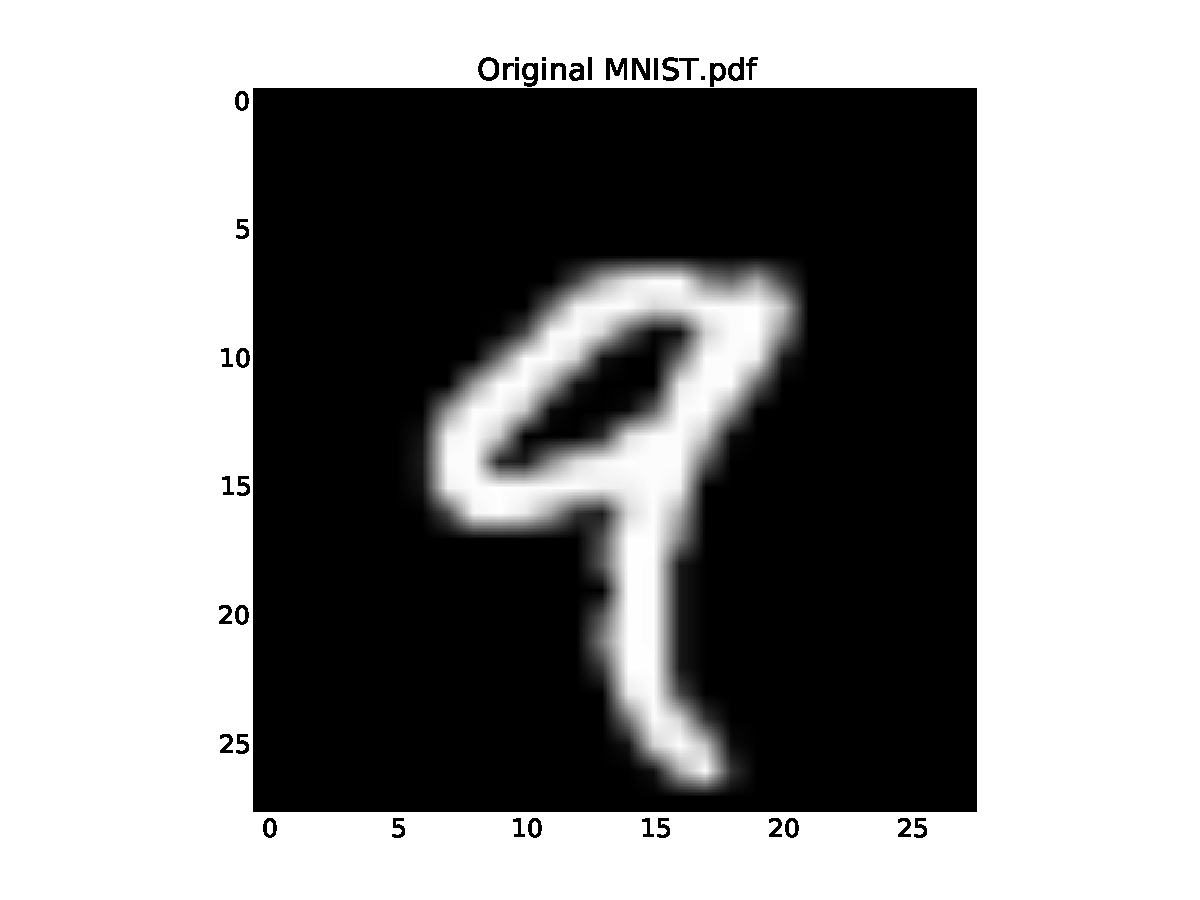
\includegraphics[scale=0.15]{OriginalMNIST.pdf}
	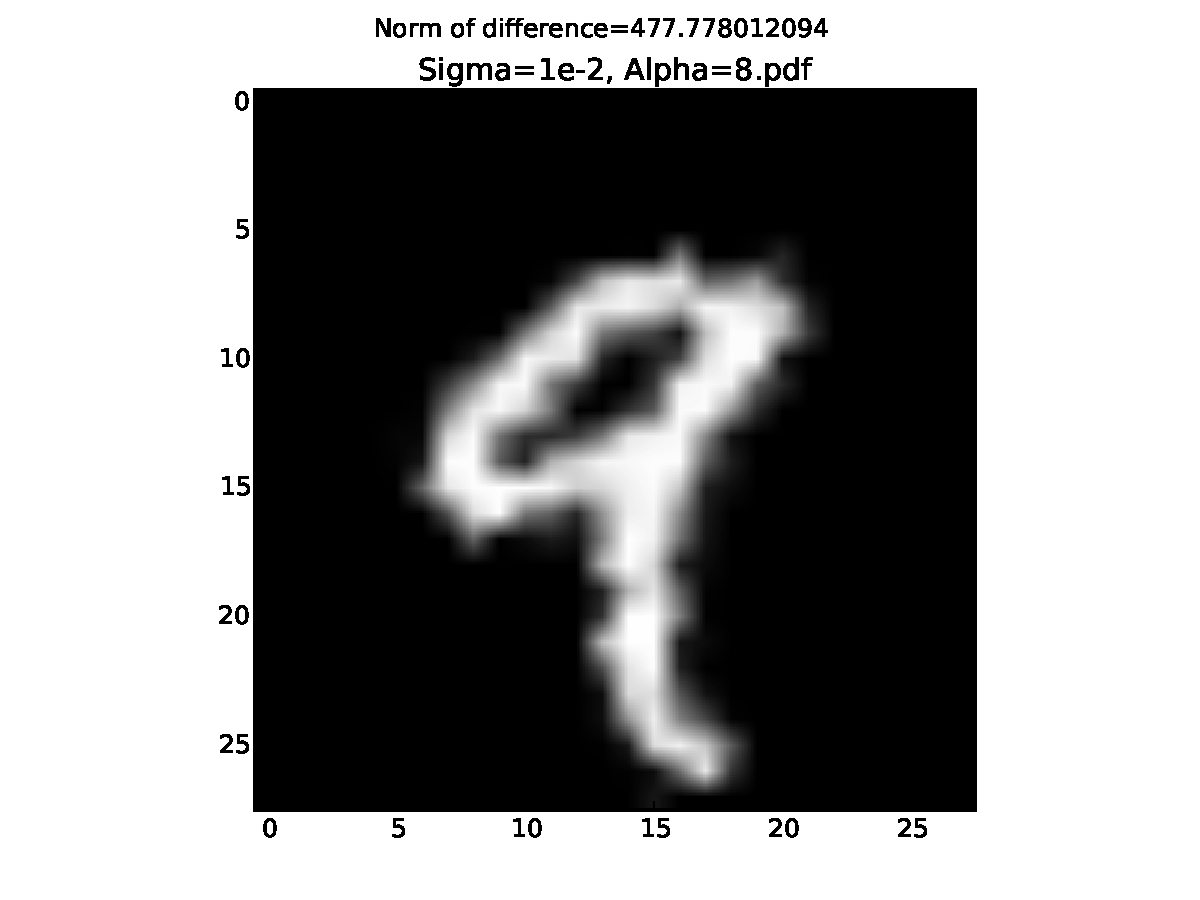
\includegraphics[scale=0.15]{Sigma=1e-2,Alpha=8.pdf}
	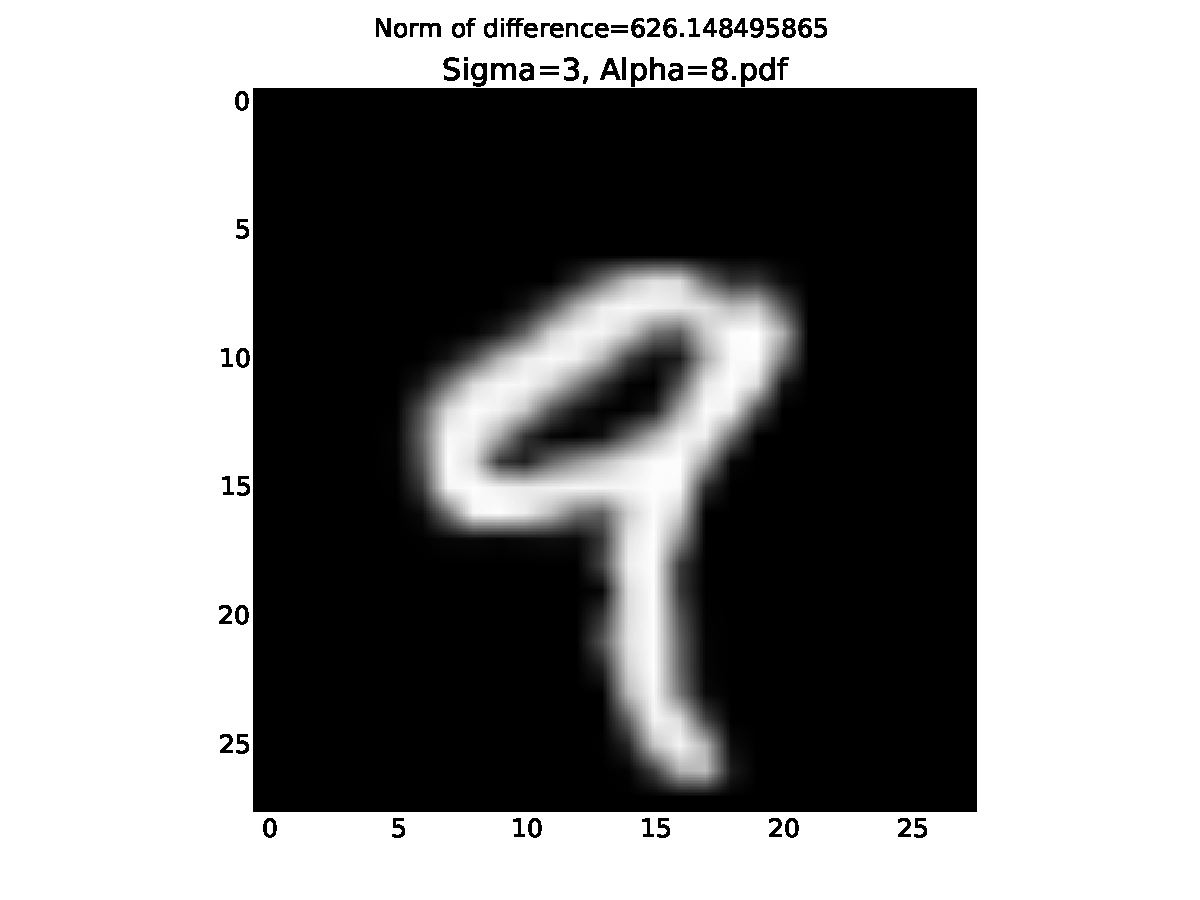
\includegraphics[scale=0.15]{Sigma=3,Alpha=8.pdf}
	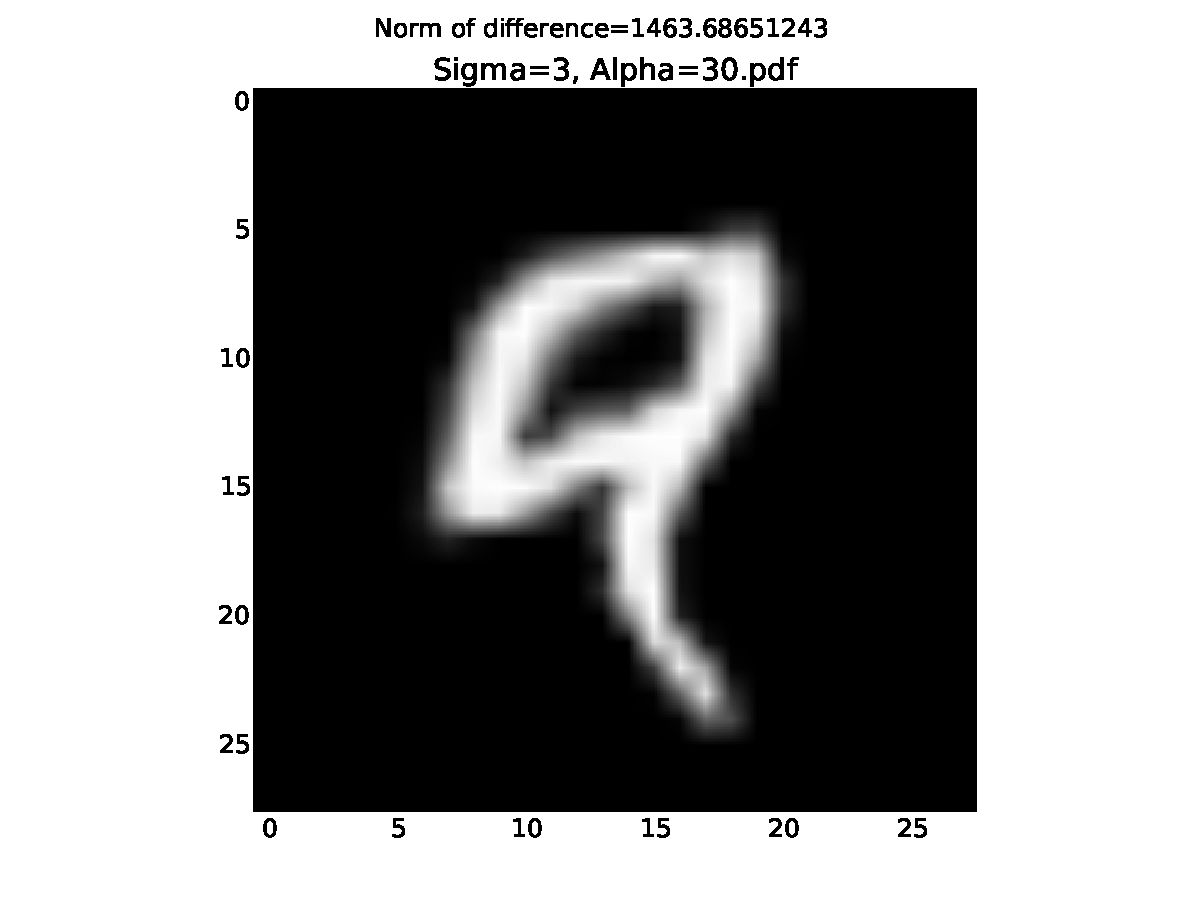
\includegraphics[scale=0.15]{Sigma=3,Alpha=30.pdf}
	\caption{The effect of varying $\sigma$ and $\alpha$}
	\label{Perturbed}
\end{figure}

The second datasource we attempted to generate, motivated by Patrice Simard et al. \cite{Simard}, involved performing an affine deformation of the modified MNIST image. 
We refer to this additional dataset as "Perturbed Modified Digits" throughout the rest of the paper. 

The methodology for generating these perturbed digits is as follows. 
Given a $n\times n$ image, we first generate two random $n\times n$ displacement fields $?x(x',y')\rightarrow uniform(-1,1)$ and $?y(x',y')\rightarrow uniform(-1,1)$. We the convolve these displacement fields by a gaussian filter with $\mu = 0$ and $\sigma$ being a variable to the function which defaults to 3. 
After this we normalize the displacement fields by dividing each element in the field by the norm of the matrix. 
All the elements in both displacement fields are then multiplied by $\alpha$ which is a variable to the function. 
We then generate a new $n\times n$ image as such: for each pixel $(i,j)$ in the original, the new value at that pixel is the value at $?x(i,j),?y(i,j)$ in the original picture. 
Bilinear interpolation is used to determine the value of $new(i,j)=original(?x(i,j),?y(i,j))$ when $?x(i,j),?y(i,j)$ are not integers. 
For indices which appear out of bounds of the picture we simply used a default value of 0. Fig \ref{Perturbed} shows the effect of varying $\alpha$ and $\sigma$ on the original MNIST dataset (similar results occur with the modified dataset, but are harder to distinguish). 
The norm of the difference between the original MNIST image and the modified image are included in the pictures. 
We found that increasing $\alpha$ causes larger smooth, deformations while decreasing $\sigma$ causes the deformation to be more random and noisy. This is consistent with the findings in the literature.



\subsection{Classification Algorithms}

\subsubsection{Baseline - Logistic Regression}
In Logistic Regression, we want to estimate the probability that some random vector $X=(x_1, \ldots, x_n)$ has a class $Y=y_k$, i.e. $P(Y=y_k | X=(x_1, \ldots, x_n))$. In the binary case we can derive the following using Bayes rule and conditioning:
\begin{equation*}
\begin{split}
&P(Y=1~|~X) = \frac{P(X, Y=1)}{P(X)}\\
&= \frac{ P(X~|~Y=1)\cdot P(Y=1) }{ P(X~|~Y=1)\cdot P(Y=1) + P(X~|~Y=0)\cdot P(Y=0) }\\
& = \sigma(a)\\
\end{split}
\end{equation*}

where $a=\ln\Big(\frac{P(Y=1~|~X)}{P(Y=0~|~X)}\Big)$ is the log-odds ratio and $\sigma (a)$ is the Sigmoid function:

\begin{equation}
	\label{sig}
	\sigma (x)= \frac{1}{1 + \exp{(-x)}} 
\end{equation}

By approximating the log-odds ratio as a linear decision boundary of the features and weights, $w^T x$ we can use this as an estimate of the class being $Y=1$. We can optimize the Log-likelihood or Cross-Entropy function:

\begin{equation}
	\label{LL}
	L(w) = -\sum_{i=1}^n y_i\log\Big(\sigma(w^Tx_i)\Big) + (1-y_i)\log\Big(1-\sigma(w^Tx_i)\Big)
\end{equation}

and search for the optimal set of weights using the \emph{gradient descent algorithm} with $K$ steps and the update rule:

\begin{equation}
\label{LR_update_rule}
	w_{k+1} = w_k + \alpha_k \sum_{i=1}^n \Big( x_i\big(y_i - \sigma(w_k^Tx_i\big) \Big)
\end{equation}

Multi-class classification was implemented using a one-vs-all approach. The choice of parameters (learning rate $\alpha$ and maximum iterations $K_\text{steps}$) was made through a 3-fold crossvalidation.

\subsubsection{Support Vector Machines}
We selected our kernel through cross validation and we tested polynomial kernels of degree 2-9, linear kernel, and a Radial Basis Function (RBF) kernel. The results can be seen in the results section. The best performing kernel, RBF kernel, isdefined as \cite{Hastie}: \[K(x,x\prime )=exp(-\gamma\|x-x\prime \|^2)\] 

where the parameter $\gamma$ corresponds to the inverse radius of influence of any training example. For examples, a low value of gamma means that an examples will have an influence on training examples far away from itself\cite{sklearn}. The penalty parameter $C$ controls the amount of allowed misclassifications, and thus the model complexity. There is usually a tradeoff between $C$ and $\gamma$. 

To select our features we broke the dataset into train, validate, and test sets with a 64, 16, 20 split. After selecting the best scoring kernel on the validation set, we performed a cross validation to pick the best $C$, $\gamma$, number of PCA components, and whether to normalize our data, on the training set plus the validation set. We then evaluated our final model on our test set.


\subsubsection{Fully Connected Feedforward Neural Network}

Neural Networks (NN) have been shown to perform very well on image classification without requiring extensive feature extraction and processing \cite{LeCun90}, as the images are fed directly into the NN. This model is advantageous for many reasons, notably as it works with low level information. The NN structure is divided into three main components: 
\begin{itemize}
\item an input layer, consisting of nodes representing an input's features, in addition to a bias node.
\item a set of hidden layers, which all include a bias node. To each node $i$ in a hidden layer is associated:
\begin{itemize}
\item $\delta_i$: the correction for node $i$
\item $w_i$: a vector representing the weight of the connection from each node in the previous layer to node $i$
\end{itemize}
\item an output layer, which in the case of multi-label classification, includes $m$ output nodes $o_1,o_2,\dots,o_m$, each representing the probability that an example belongs to class $o_j$.
\end{itemize}

The outputs of hidden and output layer nodes are calculated with an activation function. There exists many choices, one of the most common being the previously defined sigmoid function (\ref{sig}).



Learning a NN happens in 3 steps, which are repeated until convergence:
\begin{itemize}
\item \emph{Forward pass}: given an example $x$, we update a node $j$ in the first hidden layer by applying the sigmoid function to the dot product between the inputs and the weight between neurons: $$o_j=\sigma(w_j\cdot x_j)$$ We use this result as the input for the next layer until we reach the output layer.
\item \emph{Back Propagation}: we correct the weights by traversing the layers in reverse. To do so we calculate each node $j$'s share of the error, $\delta_j$ \cite{backprop}. For output neurons we have:
$$\delta_j = (y_j-o_j)o_j  (1-o_j)$$
where $y_i$ is a binary variable representing the example's membership to class $i$. For hidden neurons:
$$\delta_j=o_j (1- o_j)\left(w_j\cdot \delta_h\right)$$
where $\delta_h$ is the correction vector of the above layer.
\item \emph{Gradient Descent}: Finally, we update the weights:
$$w_j=w_j+\alpha \delta_j\cdot x_j^{\top}$$
where $\alpha$ is the learning rate.
\end{itemize}

Finally, a crucial part of the NN implementation is a good weight initialization\cite{weights}. As suggested in \cite{nndl}, we initialized weight according to a normal distribution $\mathcal{N}\left(\mu=0,\sigma=\frac{1}{\sqrt{n}}\right)$, where $n$ is the number of input weights. The intuition behind choosing this weight distribution is that it will flatten the Gaussian distribution and decrease the likelihood of neurons saturating.

\subsubsection{Convolution Neural Network}
The convolution neural network \cite{LeCunn98} is a neural network with specialized layers in which not all neurons are connected to each other. In fact the main component is the subblayer (Fig \ref{convmaxlayer}) which contains the Convolution2D and MaxPool2d pair of layers. A convolution of an image is the result where each pixel is the weighted sum of its neighbouring pixels (moving window weighted sum). This means that our 2D convolution takes a weighted sum of each neighbouring pixel of the handwritten digit. \emph{num\_filters} is the number of moving windows of size \emph{filter\_size} $\times$ \emph{filter\_size} we do convolutions with. In MaxPooling we select the maximum in a region of size \emph{pool\_size} $\times$ \emph{pool\_size} pixels obtained from the 2D convolution.


\begin{figure}[h]
	% \centering

	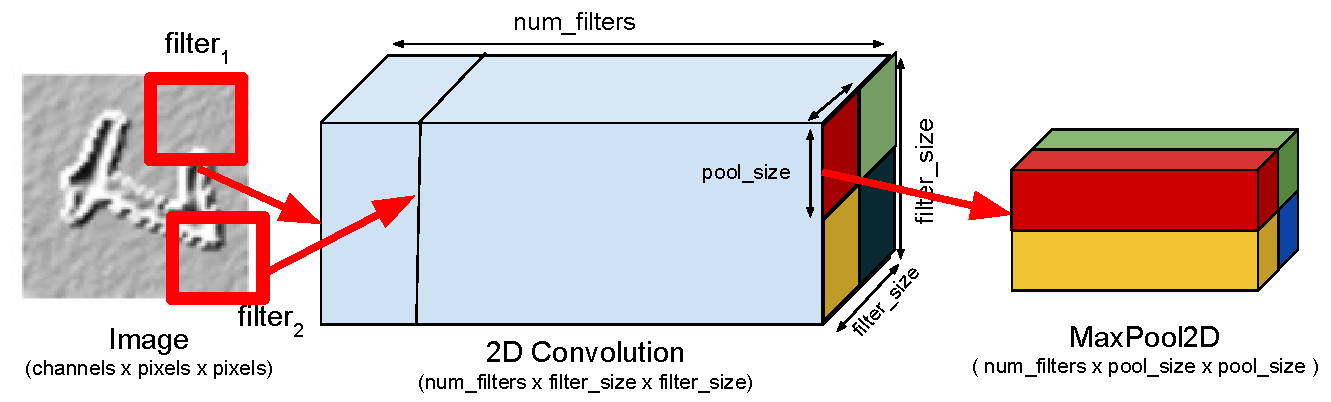
\includegraphics[scale=0.40]{convnet_example.pdf}
	\caption{A simplified example of the sublayer containing Convolution2D layer and a MaxPool2D layer. The variables correspond to the authors implementation of the network. The final network used one,two and three of these sublayers in tandem.}
	\label{convmaxlayer}
\end{figure}

As shown in the (simplified) figure \ref{convmaxlayer}, the convolution conducted on the input is transformed into the 3D spatial arrangement of the filters. This is then subsampled (by selecting the MAX element from each subsection of the filter) to produce the set of outputs that can be reused in future layers. In our architecture we stacked $K$ of the Convolution2D-Maxpool sublayers ($K=\{1,2,3,4\}$) and finally ran the outputs through a fully connected dense layer which had the same number of units as \emph{num\_filters} in the last Convolution2D-Maxpool subplayer. To obtain the final output, we ran this through a $p=0.5$ dropout and then into a fully connected dense layer of size $10$ to make the predictions. This is shown in Fig \ref{CNNarch}. 

\begin{figure}[h]
	% \centering
	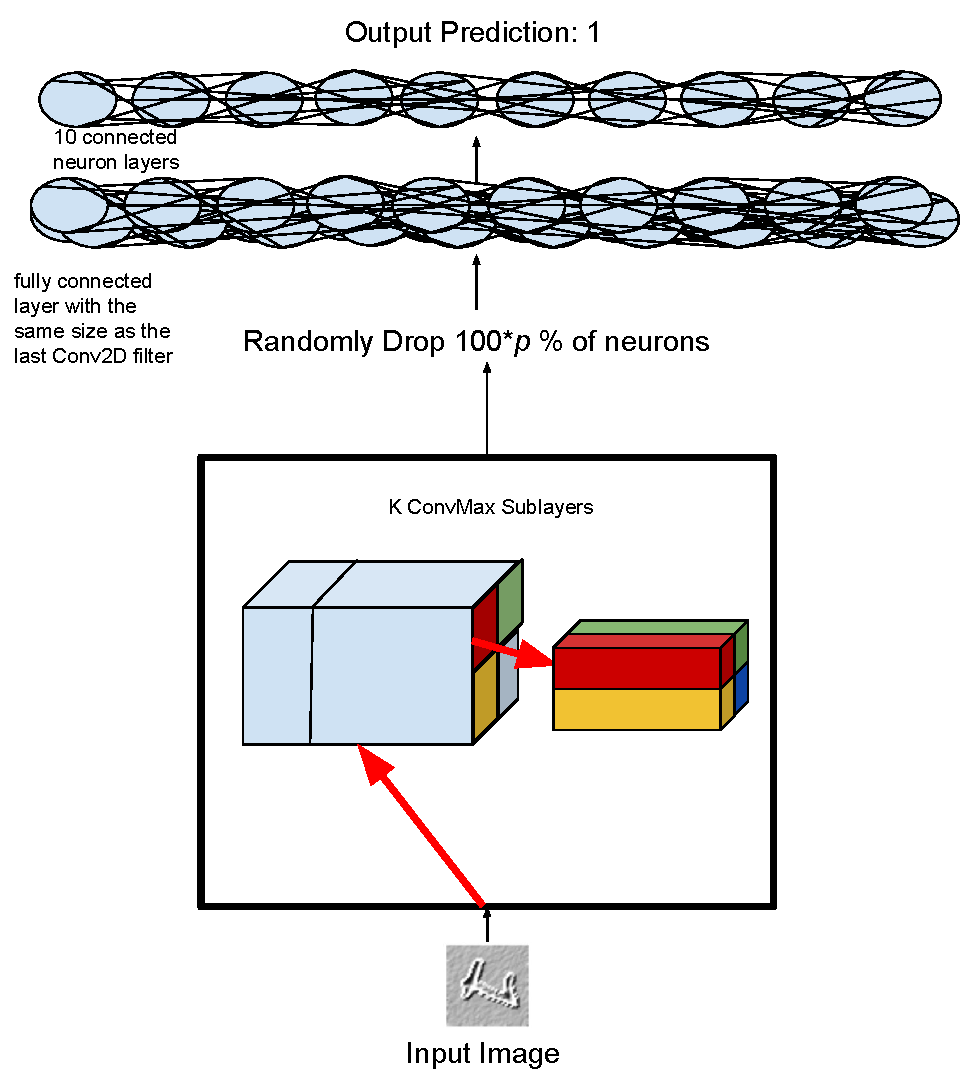
\includegraphics[scale=0.5]{architecture.pdf}
	\caption{The Convolution Neural Architechture included $k$ stacked sublayers shown in Fig \ref{convmaxlayer} connected to a dropout layer and finally fed into a fully connected layer containing $10$ neurons that did the final classification.}
	\label{CNNarch}
\end{figure}

Two methods were used to account for overfitting: (1) dropout\cite{dropout} neurons and (2) addition of extra (perturbed) data. 

In dropout, we randomly delete $50\%$ of the neurons during each forward pass and backpropagation event, which forces neurons to learn a more robust set of features. It is akin to training multiple different networks and this sampling of different neurons during the task reduces the co-dependence of neurons to make predictions. 

Adding perturbed data according to procedure IV-C, ensures that we expose our network to a wider range of possible digits. This means that the network is robust to perturbations in the data and can make better predictions in the event that there are imperfections like distortion, deletions and deformations.

\section{Results}

\subsection{Dimensionality Reduction}

Fig \ref{gridsearchpca} shows the heatmap of our GridSearch using an SVM with an RBF kernel and C=10, gamma=1e-4, we get optimal results for p=500 and normalizing the data. 

\begin{figure}[h]
	\centering
	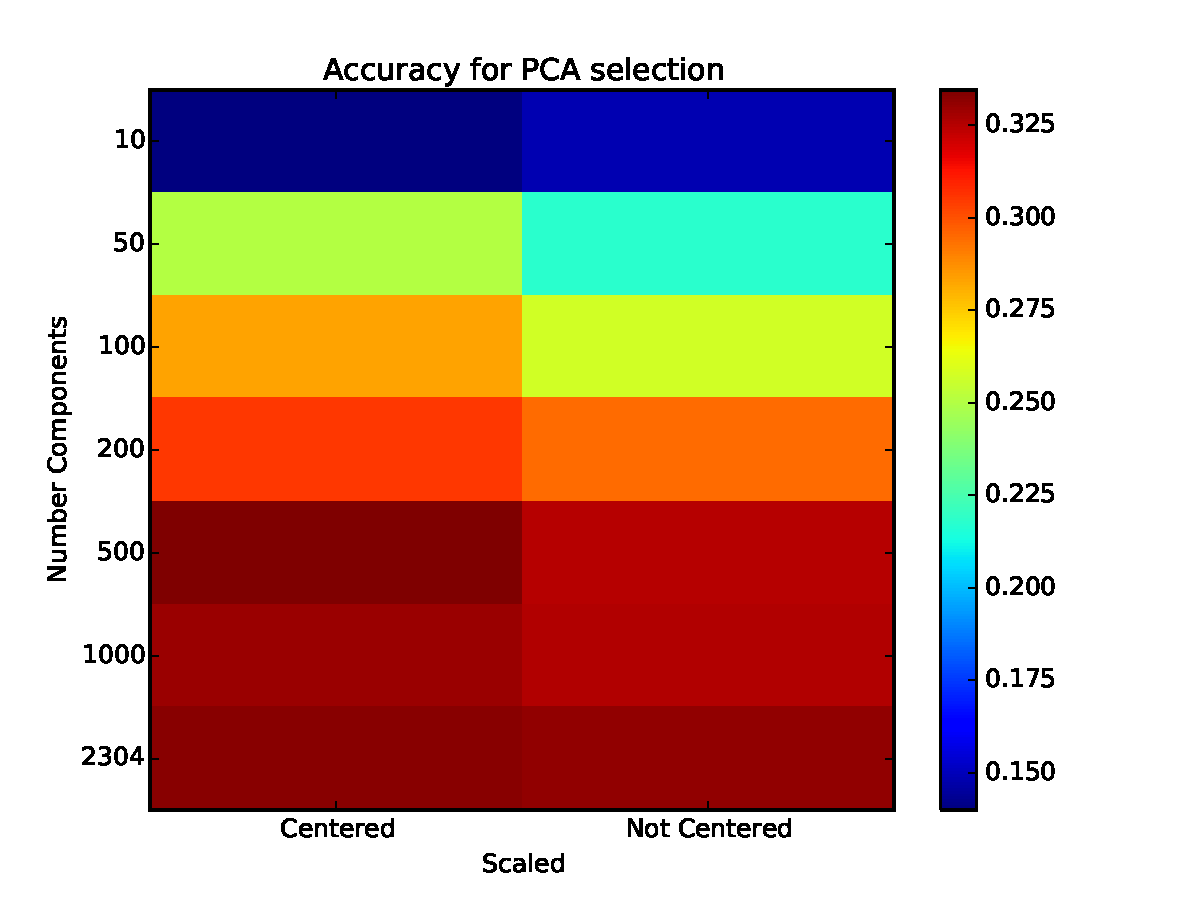
\includegraphics[scale=0.35]{PCA_gridsearch.pdf}
	\caption{The effect of varying the number of components and scaling the data}
	\label{gridsearchpca}
\end{figure}

\subsection{Logistic Regression}
The results for parameter selection are summarized in Fig \ref{LR_accuracy}. In particular the best combination of parameters are $\alpha=0.01$ and \emph{max\_iterations}=$10000$. Using this we were able to obtain a score of 0.23140 on the Kaggle leaderboard.

\begin{figure}[h]
	\centering
	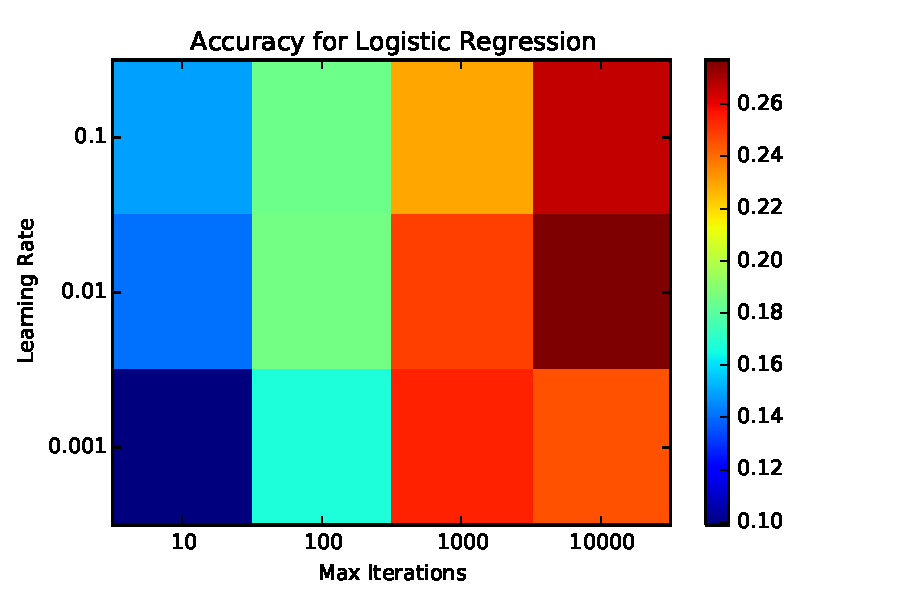
\includegraphics[scale=0.45]{LR_accuracy.pdf}
	\caption{Logistic regression cross validation results, (Red = better accuracy)}
		\label{LR_accuracy}

\end{figure}


\subsection{SVM}

As mentioned above, the best performing kernel was RBF. Performing gridsearch on SVM-RBF \ref{SVMGrid}, we found that the optimal parameter values were $C=10$ and $\gamma=10^{-4}$, which yielded an accuracy of about 33\%. 


\begin{figure}[h]
	\centering
	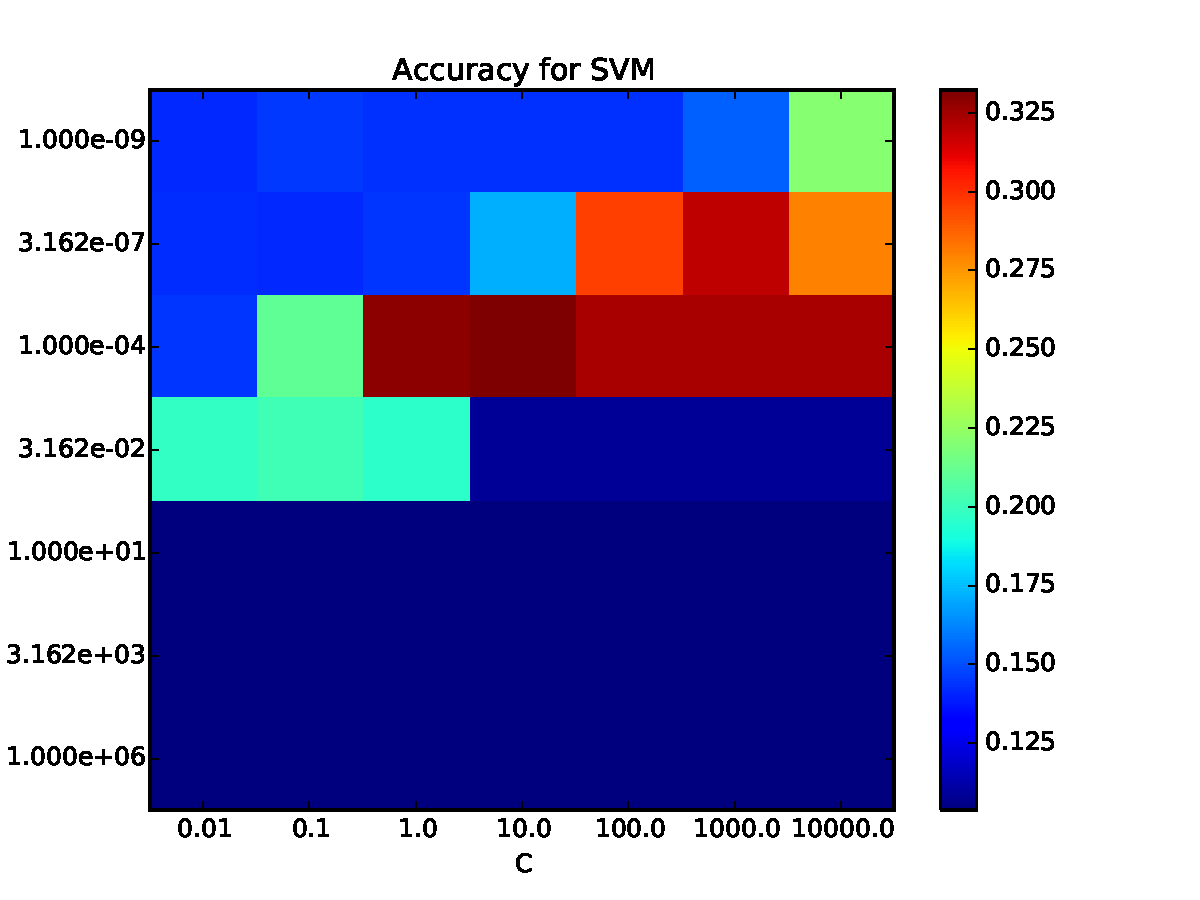
\includegraphics[scale=0.4]{SVM_grid_search.pdf}
	\caption{Heat map of SVM grid search}
	\label{SVMGrid}
\end{figure}


%\subsection{Feed-forward Neural Network}


\subsection{Convolution Neural Networks}
An epoch is one forward pass and backpropagation event. For a single Convolution-Maxpool layer, we picked the initial number of filters using two-fold cross validation to be $16$ (Fig \ref{CNNacc}). This is because using $16$ filters showed a faster increase in accuracy and selecting a smaller first filter means that there will be fewer parameters to train overall.

We then trained $2$-CNNs, $3$-CNNs and $4$-CNNs where at each additional Convolution-Maxpool layer we increase the number of filters to extract higher level features. Fig \ref{CNNacc} shows that as the depth of the network increases, we converge to higher accuracy rates.

\begin{figure}[h]
	\centering
	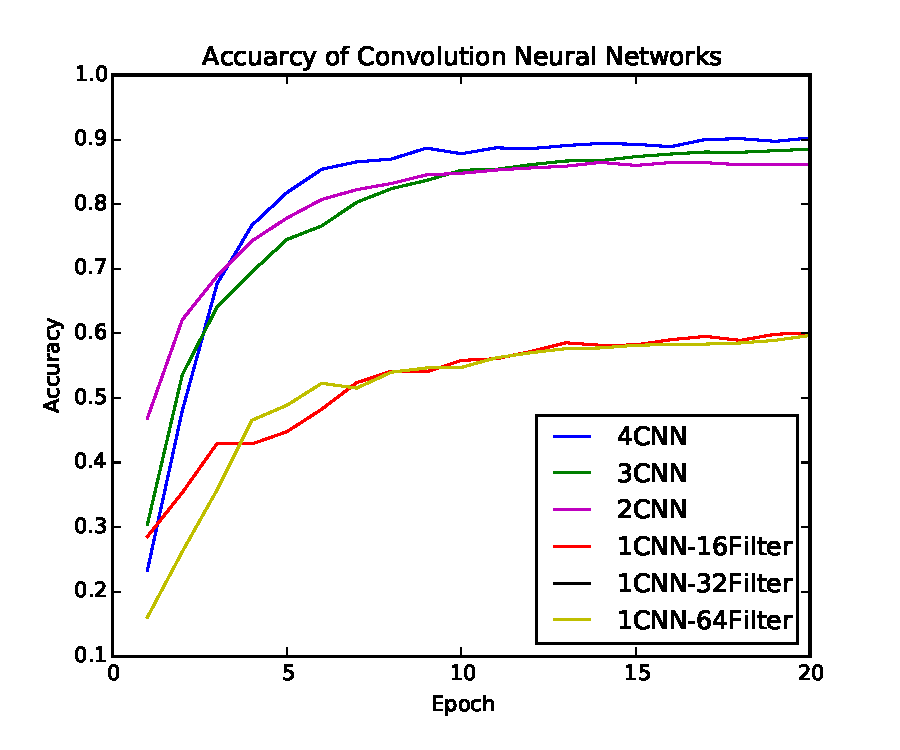
\includegraphics[scale=0.45]{CNNacc.pdf}
	\caption{Accuracy vs Epoch plot}
		\label{CNNacc}
\end{figure}

Further examination on the $4$-CNN shows that (without perturbed data) we converge to our optimal set of weights after $10-12$ epochs (Fig \ref{C4NNacc}). This prediction scored 0.90940 on the Kaggle leaderboard.

\begin{figure}[h]
	
	\centering
	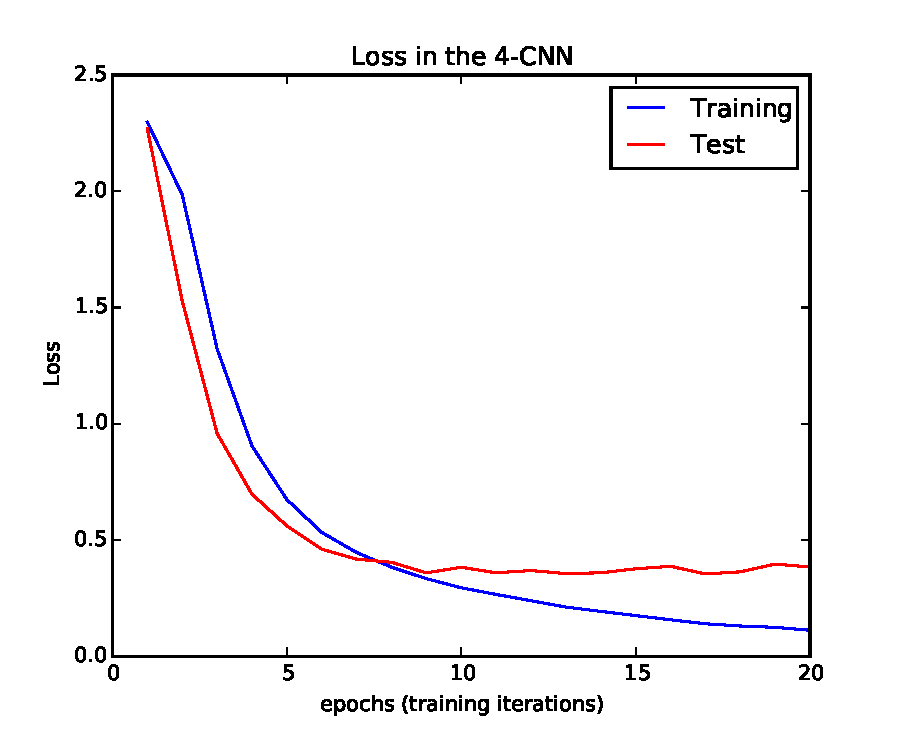
\includegraphics[scale=0.45]{4CNNloss.pdf}
	\caption{Loss in the 4CNN}
	\label{C4NNacc}
\end{figure}

As a final attempt to make our classifier more robust to unseen handwritten digits, we artificially inflated the dataset to include $50,000$ more images randomly perturbed bringing the total dataset size to $100,000$. We can compare how this classifier performs against the other $4$-CNNs in Fig \ref{CNNacc} and how quickly it converges to a solution in Fig \ref{C4NNacc}. The classifier trained with extra data scored $0.87520$ on the Kaggle leaderboard. The relative losses of both classifiers with and without extra data is found in \ref{both_C4NNacc}. Confusion matrices for each are found in Fig \ref{4CNN_confusion} (a) and (b).

\begin{figure}[h]
	
	\centering
	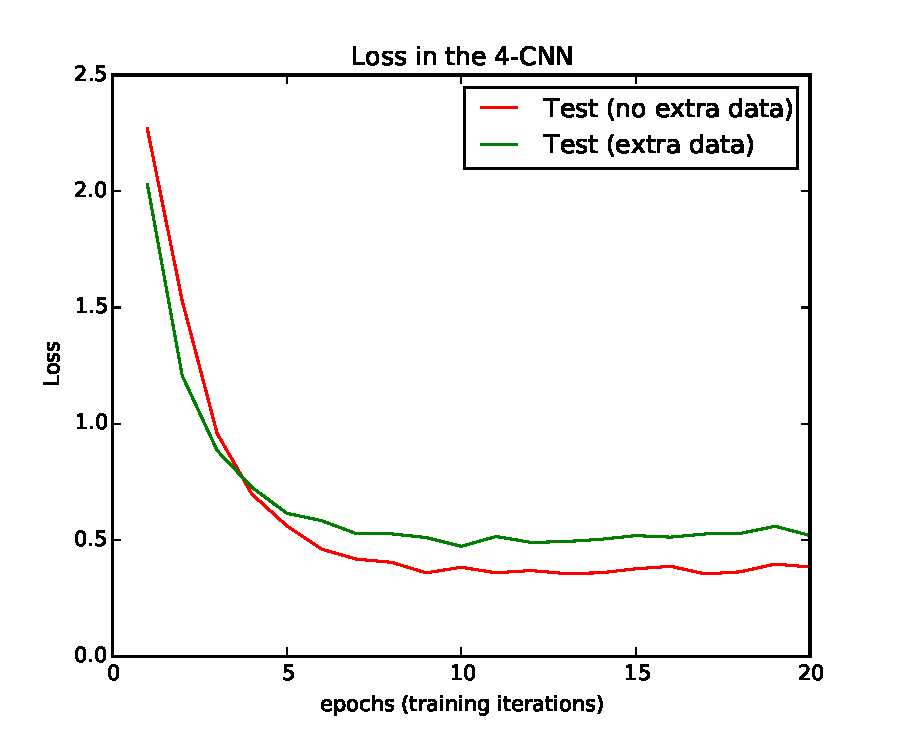
\includegraphics[scale=0.45]{4CNN_and_extraloss.pdf}
	\caption{Loss in the 4CNN both with and without extra data}
	\label{both_C4NNacc}
\end{figure}

\begin{figure}[h]
	
	\centering
	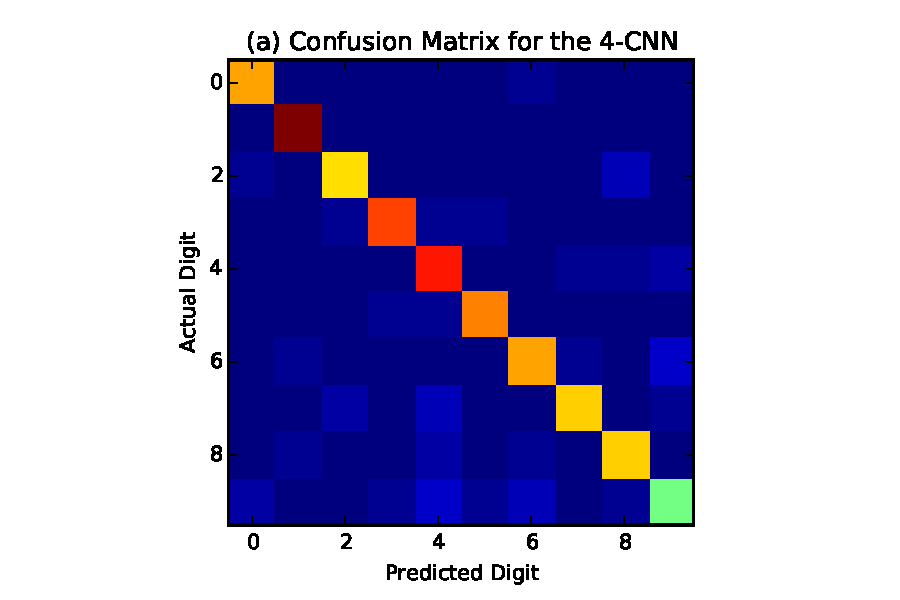
\includegraphics[scale=0.5]{4CNN_confusion.pdf}
	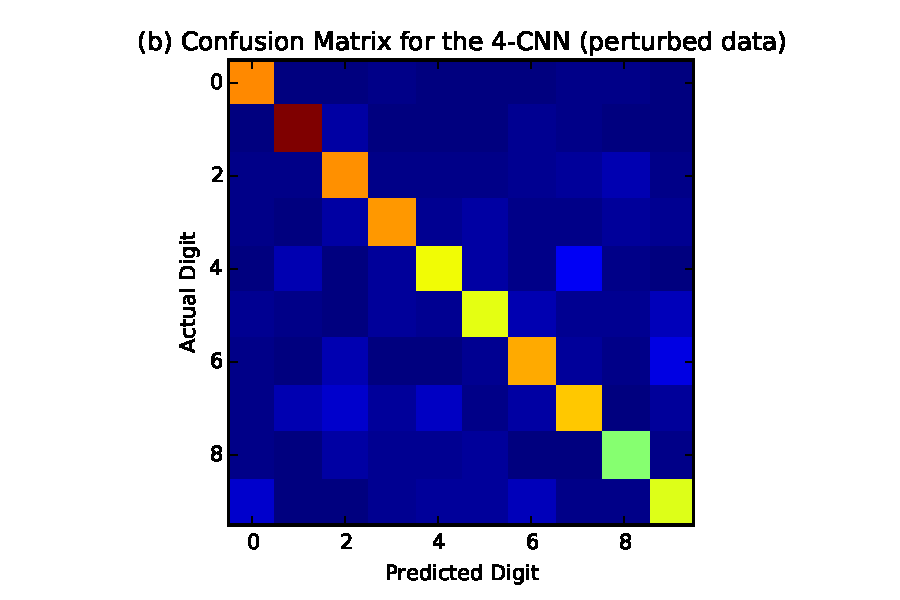
\includegraphics[scale=0.5]{4CNN_perturbed_confusion.pdf}
	\caption{Confusion Matrix for 4CNN}
	\label{4CNN_confusion}
\end{figure}


\subsection{Comparing classifiers}

The comparison of the four best classifiers is shown in Table \ref{clfs}. We can see that the $4$-CNN(Extra) outperforms the other classfiers by a significant margin.

\begin{table}[]
\centering
\caption{Classifier Performance}
\label{clfs}
\begin{tabular}{lll}
\hline
\multicolumn{1}{|l|}{\textbf{Classifier}} & \multicolumn{1}{l|}{\textbf{Parameters}} & \multicolumn{1}{l|}{\textbf{Accuracy (\%)}} \\ \hline
LogReg                                    &       $\alpha=0.01, K_{\max}=10,000$    & 23.14              \\
SVM                                       &       $C=10,\gamma=10^{-4}$        & 33.08                        \\
NN-2 layers          &       $\alpha=0.09,n_{\text{hidden}}=2,n_{\text{epochs}}=20$      &   9.60               \\
\textbf{4-CNN}                            & \textbf{$n_{\text{epochs}}=11$}   & \textbf{90.94}           \\
4-CNN(Extra)                              &             $n_{\text{epochs}}=11$        & 87.52                                      
\end{tabular}
\end{table}

\section{Discussion}

Since the data for handwritten digits is non-linear, we did not expect linear classifiers to do well on such a dataset. 

\subsection{Classifiers}

Surprisingly, all of the polynomial kernels performed as poorly as a random estimator ($\approx 10$\% accuracy). This was unexpected given the performance of the degree 9 SVM in \cite{LeCunn98}. A possible reason for this poor performance is that in order to speed up learning the number of iterations was set at a limit of 300. However, this same set up was used for the linear and RBF kernels as well and much better results were obtained with those methods. It is possible that the lack of training examples mixed with the fixed value of C (we did not perform grid search on C or gamma when picking a kernel) could have caused overfitting which would have caused the model to not generalize well.

A suprising result was the fact that a $4$-CNN trained with perturbed data did not outperform the $4$-CNN with unperturbed data. This could be due to (1) our induced perturbations not being representative of the test set or (2) limitations in our network architecture which disallowed it from learning the features more robustly. It could be that since $50\%$ of the data was perturbed and the other $50\%$ unperturbed, the classifier was unable to learn the features for each.

Table \ref{clfs} gives us a pretty good overview of which classifiers are more suited for this task. As mentioned earlier, neural networks (whether they are FFNN or 4-CNN) seem to capture the complexity of image classification. They are also advantageous as they required very little preprocessing, and should thus be a top choice when considering image classification.


\subsection{Future Work}

Regarding the generation of additional data, we would like to explore different ways of transforming the data to generate more examples. Proposed methods include adding Gaussian noise to the image, randomly setting some pixels to 0, shifting the image in some direction (the images are currently mostly centered), or overlaying some patterns similar to those used to generate the modified MNIST digits dataset. Furthermore, it would be interesting to do a comparison of how adding more data from each of these new datasets affects the train and test error of a fixed classifier. 

For the convolution neural network, we would like to further investigate the effect of adding perturbed data on our architecture. An investigation in how the proportion of perturbed data vs. unperturbed data might shine some insight into the effects of augmenting non-standard data into a dataset for prediction tasks. This will be a useful experiment as it will try to understand how a dataset composed from different data sources affects a classifiers performance versus a classifier trained on data from only one source.

Next steps involve investigation into a "Spatial Transformer Network" \cite{STN} and see how it compares to the industry standard Convolution Neural Network used in this paper. In this novel network, rotations and resizing are explicitly taken care of by a special "Transformer" layer that will \emph{undo} modifications on a digit. 


\section{Statement of Contributions}

\begin{enumerate}
\item D.R. wrote preprocessing and perturbation algorithms to create more sample points. D.R. also wrote and conducted grid search experiments using the Support Vector Machine.
\item Z.A. wrote the Logistic Regression classifier from scratch. Z.A. also developed the Convolution Neural Network Architecture and ran experiments to cross validate different layering approaches.
\item P.G. wrote the Feed-Forward Neural Network from scratch. P.G. also wrote data analysis scripts and conducted experiments using the Feed-Forward Neural Network.
\item All authors contributed equally to the generation of this report, including graphics.
\end{enumerate}


\section{Integrity of work}
We hereby state that all the work presented in this report is that of the authors.
\begin{thebibliography}{9}

\bibitem{FaceNet}
Schroff F., Kalenichenko D., Philbin J.
\emph{FaceNet: A Unified Embedding for Face Recognition and Clustering}
2015

\bibitem{MNIST_Original}
LeCun Y., Cortes, C. and Burges C.J.C.
	\emph{The MNIST Database of handwritten digits}
	http://yann.lecun.com/exdb/mnist/
% inspiration for graphic http://cs231n.github.io/convolutional-networks/


\bibitem{LeCunn98}
LeCun Y., Bengio Y., and Haffner P.
 \emph{Gradient-Based Learning Applied to Document Recognition}
 Proceedings of the IEEE,
 1998.

\bibitem{modifiedMNIST}
Carrier P.L.
\emph{Leveraging noisy side information for disentangling of factors of
variation in a supervised setting} (thesis)
2014


\bibitem{LeCun90}
  LeCun Y. et al.
  \emph{Handwritten Digit Recognition with a Back-Propagation Network}
    Advances in Neural Information Processing Systems (NIPS)
    1990

\bibitem{Hastie}
 Hastie T., Tibshirani R. Friedman J.
 \emph{The Elements of Statistical Learning: Data Mining, Inference, and Prediction}.
2nd edition
2009

\bibitem{weights}
Bengio Y.
\emph{Practical Recommendations for Gradient-Based Training of Deep Architectures}
2012

\bibitem{CNN_committees}
 Claudiu D. and Meier U. et al.
  \emph{Convolutional Neural Network Committees For Handwritten Character
Classification}
  ACM Computing Surveys (CSUR) 34
  2002.

  
\bibitem{Simard}
  Simard F., Steinkraus D., Platt J.
  \emph{Best Practices for Convolutional Neural Networks
Applied to Visual Document Analysis}
	Microsoft
    http://research.microsoft.com/pubs/68920/icdar03.pdf.


\bibitem{sklearn}
Pedregosa F., Varoquaux G., Gramfort A., et al.
\emph{Scikit-learn: Machine Learning in {P}ython}
Journal of Machine Learning Research    
Vol 12, 2825-2830 2011   

\bibitem{nndl}
Nielsen M.
\emph{Neural Networks and Deep Learning}
Available online at: \href{http://neuralnetworksanddeeplearning.com/}{http://neuralnetworksanddeeplearning.com/}
2015       

\bibitem{dropout}
Krizhevsky A., Sutskever I., and Hinton G.E.
\emph{ImageNet Classification with Deep Convolution Neural Networks}
	NIPS 2012

\bibitem{backprop}
	Irena Koprinska's notes on neural networks backpropagation.
	http://sydney.edu.au/engineering/it/~comp4302/ann4-6s.pdf
	Accessed on the web on 11/11/2015

\bibitem{STN}
 Jaderberg, M., et al.
  \emph{Spatial Transformer Networks}
  ArXiv
  2015

\end{thebibliography}

\end{document}
